\documentclass[type=bachelor]{thuthesis}
% 选项:
%   type=[bachelor|master|doctor|postdoctor], % 必选
%   secret,                                   % 可选
%   pifootnote,                               % 可选(建议打开)
%   openany|openright,                        % 可选,基本不用
%   arial,                                    % 可选,基本不用
%   arialtoc,                                 % 可选,基本不用
%   arialtitle                                % 可选,基本不用

% 所有其它可能用到的包都统一放到这里了,可以根据自己的实际添加或者删除。
\usepackage{thuthesis}
\usepackage{bm}
\newcommand{\transpose}[1]{\ensuremath{#1^{\scriptscriptstyle T}}}
\DeclareMathOperator*{\rgmax}{argmax}
\DeclareMathOperator*{\rgmin}{argmin}
\DeclareMathOperator{\Tr}{Tr}
% 定义所有的图片文件在 figures 子目录下
\graphicspath{{figures/}}

% 可以在这里修改配置文件中的定义。导言区可以使用中文。

\begin{document}

%%% 封面部分
\frontmatter
\thusetup{
  %******************************
  % 注意:
  %   1. 配置里面不要出现空行
  %   2. 不需要的配置信息可以删除
  %******************************
  %
  %=====
  % 秘级
  %=====
  secretlevel={秘密},
  secretyear={10},
  %
  %=========
  % 中文信息
  %=========
  ctitle={无线网络中定位信息的时空传播机理研究},
  cdegree={理学学士},
  cdepartment={数学科学系},
  cmajor={数学与应用数学},
  cauthor={赵丰},
  csupervisor={沈渊\quad 副教授},
  cassosupervisor={梁恒\quad 副教授}, % 副指导老师
  ccosupervisor={某某某教授}, % 联合指导老师
  % 日期自动使用当前时间,若需指定按如下方式修改:
  % cdate={超新星纪元},
  %
  % 博士后专有部分
  cfirstdiscipline={计算机科学与技术},
  cseconddiscipline={系统结构},
  postdoctordate={2009年7月——2011年7月},
  id={编号}, % 可以留空: id={},
  udc={UDC}, % 可以留空
  catalognumber={分类号}, % 可以留空
  %
  %=========
  % 英文信息
  %=========
  etitle={An Introduction to \LaTeX{} Thesis Template of Tsinghua University v\version},
  % 这块比较复杂,需要分情况讨论:
  % 1. 学术型硕士
  %    edegree:必须为Master of Arts或Master of Science(注意大小写)
  %             “哲学、文学、历史学、法学、教育学、艺术学门类,公共管理学科
  %              填写Master of Arts,其它填写Master of Science”
  %    emajor:“获得一级学科授权的学科填写一级学科名称,其它填写二级学科名称”
  % 2. 专业型硕士
  %    edegree:“填写专业学位英文名称全称”
  %    emajor:“工程硕士填写工程领域,其它专业学位不填写此项”
  % 3. 学术型博士
  %    edegree:Doctor of Philosophy(注意大小写)
  %    emajor:“获得一级学科授权的学科填写一级学科名称,其它填写二级学科名称”
  % 4. 专业型博士
  %    edegree:“填写专业学位英文名称全称”
  %    emajor:不填写此项
  edegree={Doctor of Engineering},
  emajor={Computer Science and Technology},
  eauthor={Xue Ruini},
  esupervisor={Professor Zheng Weimin},
  eassosupervisor={Chen Wenguang},
  % 日期自动生成,若需指定按如下方式修改:
  % edate={December, 2005}
  %
  % 关键词用“英文逗号”分割
  ckeywords={协作定位,费舍尔信息矩阵,定位误差下界,矩阵代数,连分式},
  ekeywords={\TeX, \LaTeX, CJK, template, thesis}
}

% 定义中英文摘要和关键字
\begin{cabstract}
  对于目标的实时位置的获取是无线通信技术的应用的重要一部分。在有多个目标节点的定位场景下,利用目标节点之间相互通信得到的距离信息的协作定位技术对定位精度的提高有显著的作用。随着定位网络规模的扩大和时间上的延长,各种测量数据如何影响定位误差是本文要研究的内容。

  本文从高斯测量信号模型出发,从费舍尔信息矩阵的角度刻化了定位误差的时空衰减特性。在数学方法方面,本文主要运用了矩阵代数的运算规则推导了费舍尔信息矩阵特征值的闭式表达式,并运用函数的连分式展开的分析方法求出了定位误差的时空衰减速度的量阶,从而揭示了定位误差与协作信息的关系的一般机理。

  在本文的研究工作中比较突出的一点在于,本文在单节点时间协作问题上得出了一般情形下误差下界的连分式表达形式,并且在理论上证明了采样时间间隔趋于零时的误差下界和节点的运动轨迹无关的性质,这对于单节点路径规划与运动控制有一定的理论指导意义。
\end{cabstract}

% 如果习惯关键字跟在摘要文字后面,可以用直接命令来设置,如下:
% \ckeywords{协作定位,费舍尔信息矩阵, 定位误差下界,矩阵代数,连分式}

\begin{eabstract}
    Translation of the chinese abstract.
\end{eabstract}

% \ekeywords{\TeX, \LaTeX, CJK, template, thesis}

% 如果使用授权说明扫描页,将可选参数中指定为扫描得到的 PDF 文件名,例如:
% \makecover[scan-auth.pdf]
\makecover

%% 目录
\tableofcontents

%% 符号对照表
\begin{denotation}[3cm]
\item[$N_b$] 锚点数量
\item[$\bm{p}_i$] 第i个待定位节点的位置,在时间协作中表示目标节点各个时刻的位置
\item[$\bm{P}$] 全部要估计的待定位节点的位置向量,即$(\bm{p}_1,\bm{p}_2,\dots,\bm{p}_{N_a})$
\item[$\bm{p}^b_i$] 第i个锚点的位置
\item[$f(x_1,\dots,x_n|\theta)$] 参数$\theta$已知条件下随机变量$X_1,\dots,X_n$联合概率密度函数
\item[$\bm{I}(\bm{p})$] 关于待定位节点位置$\bm{p}$的费舍尔信息矩阵
\item[$N_a$] 待定位节点数量,在时间协作中表示采样的数量
\item[$\sigma^2_{i}$] 待定位节点和锚点i之间测距的方差
\item[$\sigma^2_{i,j}$] 节点i和节点j之间测距的方差
\item[$\bm{u}_{i,j}$] 节点i和节点j之间的单位方向向量,时间协作中表示采样时刻$t_i$和$t_j$之间目标节点的位置变化向量
\item[$\bm{C}_{i,j}$] 费舍尔信息矩阵位于i行j列的元素的相反数
\item[$\Delta t$] 时间协作中采样时间间隔
\item[$\lambda_{i}$] 表示$\sigma^2_{i}$的倒数
\item[$\bm{u}_i$] 待定位节点和锚点i之间的单位方向向量,时间协作中表示第i个时刻的位置和第i+1个时刻的位置之间的单位方向向量
\item[$\phi_i$] $\bm{u}_i$的方向角,时间协作中表示第$t_i$时刻$\bm{u}_{i,i+1}$的方向角
\item[$\bm{A}^{-1}_{1\times2,1\times2}$] 方阵$\bm{A}$的逆阵由前两行和前两列决定的子矩阵
\end{denotation}



%%% 正文部分
\mainmatter
\chapter{引言}
\label{cha:intro}

\section{研究背景}
%background info here
对于目标的实时位置的获取是无线通信技术的应用的重要一部分,其在车辆导航与编队、军事演习等方面有着广泛的应用前景。


%tech info here
通常一个无线定位系统可以依赖于GPS卫星定位,但在室内定位的场合,由于微波被建筑物散射等原因,定位效果并不理想,在这种情况下需要根据应用的场景开发
地面无线定位系统。通常一个地面无线定位系统会事先部署一些位置已知的锚点(基站)采用某个特殊的频段的电磁波与位置未知的目标节点进行通信,在锚点处可以通过测量无线信号到达的时间或信号强度等信息估计出某个基站与场景中目标节点的距离,如果是对目标的追踪也会利用上前一个时刻得到的定位结果,利用统计学的方法对这些数据进行实时的处理,可以估计出目标节点的位置或运动的轨迹。


%non-cooperative case to cooperative case
传统的定位方法是只利用锚点和目标节点彼此之间的测距信息对目标节点进行定位,在有多个目标节点的定位场景下,随着技术的成熟近年来发展出了利用目标节点之间相互通信得到的距离信息的协作定位技术,协作定位技术不仅利用了目标节点和已知位置的锚点之间的信息,还利用了目标节点彼此之间的定位信息,从而提高了定位精度。


%algorithm property analysis
协作定位技术已经有了一定的研究基础,目前已经有大量的文献针对定位算法展开探讨,对定位算法的性能研究一般可以通过理论推导和仿真比较等方法,在理论
推导方面,已经得出了在给定的定位场景(定位网络)下存在一个统计平均意义上的定位误差下界\cite{LimitBound},任何基于测量数据对目标节点的位置估计的误差都在这个定位误差下界之上。因此研究和分析这个定位误差下界随着定位网络规模的扩大和采样时间间隔的缩短对于定位算法的设计具有一定的指导意义。

\section{研究问题}
%content
在本人的研究中,我会首先建立定位网络的数学模型并根据建立的模型推导定位误差下界的一般表达式,然后分别针对若干特殊的定位网络推导误差下界的解析表达式,并根据解析表达式分析定位性能随网络的时空规模的变化规律。

%focus
\section{文章结构}
本文的研究重点是特殊定位网络误差下界的推导,在(\ref{section:model})一节中给出了问题的数学模型,主要分非协作定位场景(\ref{subsection:noncooperative_localization})、空间协作定位场景(\ref{subsection:cooperative_localization})、时间协作定位场景(\ref{subsection:temporal_cooperative_localization})三部分,(\ref{subsection:model_discussion})小节中对模型的合理性进行了进一步讨论。
在(\ref{section:research_content})一节中分别对上一节提出的数学模型进行求解,其中非协作情形(\ref{subsection:circle_general})针对小节(\ref{subsection:noncooperative_localization})的模型,空间两个节点协作(\ref{subsection:two_node_cooperation})、N个节点两两协作(\ref{subsection:complete_graph_cooperation})、大规模正方形和正六边形网络协作(\ref{subsection:square_and_hexagon_network})
针对(\ref{subsection:cooperative_localization})的模型,一个节点时间上的协作(\ref{subsection:linear_network})针对(\ref{subsection:temporal_cooperative_localization})的模型。
最后(\ref{section:conclusion})一节对全文使用的数学方法和取得的成果进行了总结,
\chapter{研究内容}
\label{cha:content}

\section{问题的数学模型}

\subsection[非协作定位场景]{非协作定位场景}

{单个节点定位}

        考虑一个平面定位场景中部署了$N_b$个位置已知的\textcolor{blue}{锚点},锚点的位置记为$\{\bm{p}^b_1,\bm{p}^b_2,...\bm{p}^b_{N_b}\}$,现在要对场景中一个\textcolor{blue}{位置未知}的节点进行定位,待定位节点的位置为$\bm{p}$,如图(\ref{fig:non_cooperative_spatial})所示。
        \begin{figure}
          \centering
          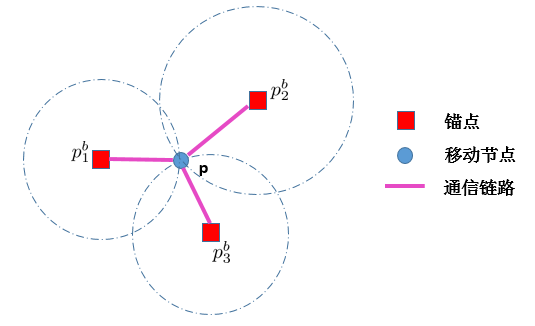
\includegraphics[width=300pt]{non_cooperative_spatial.png}
          \caption{非协作静态场景下的定位}\label{fig:non_cooperative_spatial}
        \end{figure}
假设\textcolor{blue}{待定位节点}和每一个锚点都可以相互通信进行无线测距,距离测量量服从均值为$||\bm{p}^b_i-\bm{p}||$,方差为$\sigma_i$的正态分布$X_i$。

$N_b$个\textcolor{blue}{独立}测量量的联合概率分布为:
\begin{equation}\label{eq:single}
f(x_1,...x_{N_b}|\textbf{p})=\prod_{i=1}^{N_b}\frac{1}{\sqrt{2\pi\sigma_i^2}}exp(-\frac{(x_i-||\bm{p}^b_i-\bm{p}||)^2}{2\sigma_i^2})
\end{equation}

根据点估计的理论,对于一个无偏估计量,它的方差的下界是\textcolor{blue}{费舍尔信息量}(Fisher Information)的倒数,称之为\textcolor{blue}{克拉美罗界}(Crame Rao Bound)。
  % - A title should summarize the slide in an understandable fashion
  %   for anyone how does not follow everything on the slide itself.


{费舍尔信息矩阵}
以节点的\textcolor{blue}{2维}位置为待估计参数,费舍尔信息量推广为\textcolor{blue}{费舍尔信息矩阵}(Fisher Information Matrix)。

对于我们的模型问题,费舍尔信息矩阵有如下的形式:
\begin{equation}\label{eq:uu}
I(\bm{p})=\displaystyle\sum_{i=1}^{N_b}\frac{1}{\sigma_i^2}\bm{u}_i\bm{u}_i^T
\end{equation}
其中
\begin{equation}
\bm{u_i}=\frac{\bm{p}^b_i-\bm{p}}{||\bm{p}^b_i-\bm{p}||}
\end{equation}


\subsection[协作定位场景]{协作定位场景}

{多个待测节点协作定位}
考虑一个平面定位场景中不仅部署了$N_b$个位置已知的锚点,还有$N_a$个位置未知的待定位节点,某些位置未知的节点之间可以\textcolor{blue}{彼此测距},如图(\ref{fig:cooperative_spatial})所示。第i和第j个未知节点距离测量量服从均值为$||\bm{p}^a_i-\bm{p}^a_j||)$,方差为$\sigma_{ij}$的正态分布$X_{ij}$。
        \begin{figure}
          \centering
          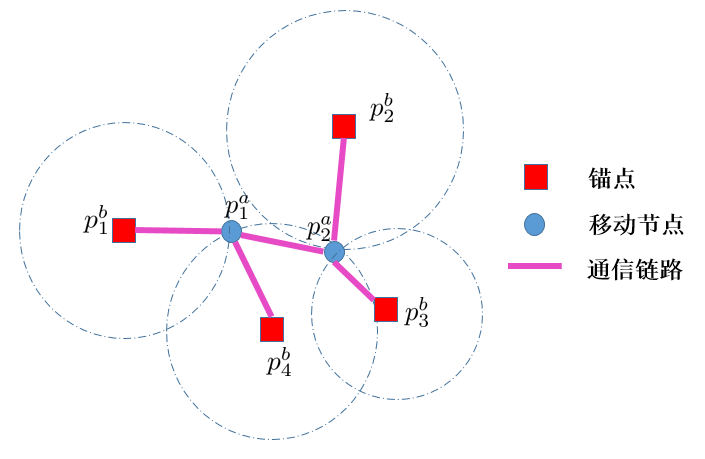
\includegraphics[width=300pt]{cooperative_spatial.png}
          \caption{协作静态场景下的定位}\label{fig:cooperative_spatial}
        \end{figure}

以$N_a$个未知节点的位置$\{p_i^a\}$作为待估计的参数,可以得到测距量的联合概率密度函数为

\begin{equation}
\prod_{i=1}^{N_a} f(x^i_1,...x^{i}_{N_b}|\bm{p^a_i})\prod_{(i,j)\in \mathcal{E}}\frac{1}{\sqrt{2\pi\sigma_{ij}^2}}exp(-\frac{(x_{ij}-||\bm{p}^a_i-\bm{p}^a_j||)^2}{2\sigma_{ij}^2})
\end{equation}
上式中f的具体表达式为式(\ref{eq:single}),$\mathcal{E}$表示可以彼此测距的未知节点的二元组的集合,而$x_t^i$表示第t个锚点和第i个未知节点的距离测量量。

\textbf{费舍尔信息矩阵}
仿照单节点时费舍尔信息矩阵的推导,关于$2N_a$个参数$\{p_i^a\}$的费舍尔信息矩阵有如下的表达形式:
\begin{equation}
\scriptsize{
I(\bm{P})=
\left(
\begin{array}{cccc}
I_B(\bm{p}_1)+&-\bm{C}_{1,2}&...&-\bm{C}_{1,N_a}\\
\sum_{j\in \{1,..N_a\}\backslash\{1\}}\bm{C}_{1,j}&&&\\
&&&\\
-\bm{C}_{1,2} & I_B(\bm{p}_2)+
&...&-\bm{C}_{2,N_a}\\
&\sum_{j\in \{1,..N_a\}\backslash \{2\}}\bm{C}_{2,j}&&\\
&&&\\
\vdots &\vdots&\ddots &\vdots\\
&&&\\
&&&I_B(\bm{p}_{N_a})+\\
-\bm{C}_{1,N_a}&-\bm{C}_{2,N_a}&...& \sum_{j\in \{1,..N_a\}\backslash\{N_a\}}\bm{C}_{N_a,j}\\
\end{array}
\right)
}
\end{equation}
上面的式子中$I_B(\bm{p}_i)$表示$N_b$个锚点对未知节点距离测量的贡献,和前面的(\ref{eq:uu})式相同。$C_{i,j}=\bm{1}_{(i,j)\in E}\bm{u}_{ij}\bm{u}_{ij}^T/\sigma^2_{ij}$,表示未知节点i和j协作的矩阵。
$\bm{u}_{ij}=\frac{\bm{p}^a_i-\bm{p}^a_j}{||\bm{p}^a_i-\bm{p}^a_j||}$表示未知节点i和j的方向向量。
\subsection[时间协作定位]{时间协作定位}

{单个待测节点时间协作定位}
考虑一个平面定位场景中有一个待定位的移动节点,场景中部署的$N_b$个位置已知的锚点分别在在$t_1,\dots,t_{N_a}$时刻对该节点进行定位,移动节点可以通过自身的加速度传感器对自己的速度有测量,如图(\ref{fig:cooperative_single_temporal})所示。
        \begin{figure}
          \centering
          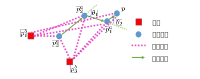
\includegraphics[width=300pt]{cooperative_single_temporal.png}
          \caption{协作静态场景下的定位}\label{fig:cooperative_single_temporal}
        \end{figure}

假设测量时间间隔比较小使得相邻测量间节点速度方向可近似看作不变,速度测量值服从均值为$v$,方差为$\sigma_{v}$的正态分布$V_{ij}$。
那么以节点各时刻的的位置$\{p_i\}$作为待估计的参数,可以得到包括相邻时刻间的所有测距量的联合概率密度函数为
\begin{equation}\label{eq:single}
\prod_{i=1}^{N_a} f(x^i_1,...x^{i}_{N_b}|\bm{p^a_i})
\prod_{i=1}^{N_a-1}\frac{1}{\sqrt{2\pi}\sigma_v(t_{i+1}-t_i)}
exp(-\frac{(v_{i,i+1}(t_{i+1}-t_i)-||\bm{p}^i-\bm{p}^{i+1}||)^2}{2\sigma_v^2(t_{i+1}-t_i)^2})
\end{equation}
{费舍尔信息矩阵}
关于$2N_a$个参数$\{p_i^a\}$的费舍尔信息矩阵有如下的表达形式:
\begin{equation}\label{eq:time_cooperation_matrix}
\scriptsize{
I(\bm{P})=
\left(
\begin{array}{ccccc}
I_B(\bm{p}_1)+\bm{C}_{1,2}&-\bm{C}_{1,2}&\bm{0}&\dots&\bm{0}\\
&&&&\\
-\bm{C}_{1,2} & I_B(\bm{p}_2)+\bm{C}_{1,2}+\bm{C}_{2,3}&-\bm{C}_{2,3}&\dots&\bm{0}\\
\vdots &\vdots&\ddots &\vdots&\vdots\\
&&&&\\
\bm{0}&\bm{0}&...& -\bm{C}_{N_a-1,N_a}&\bm{C}_{N_a-1,N_a}+I_B(\bm{p}_{N_a})\\
\end{array}
\right)
}
\end{equation}
上面的式子中若将2乘2的矩阵看作单位元素,则是一个三对角的矩阵。$I_B(\bm{p}_i)$表示$N_b$个锚点对未知节点距离测量的贡献,和前面的(\ref{eq:uu})式相同。$C_{i,i+1}=\bm{1}_{(i,j)\in E}\bm{u}_{ij}\bm{u}_{ij}^T/(\sigma_v^2(t_{i+1}-t_i)^2)$,表示未知节点i和j协作的矩阵,$\bm{u}_{ij}$表示未知节点i和j的方向向量。
\subsection{关于模型的讨论}
上面三小节给出了三种典型的定位场景,我们还需要如下限制条件模型才比较合理:
\begin{itemize}
  \item 如果测量误差$\sigma$有一个最小的阀值的话,部署的锚点不能离目标节点太近以及多个目标节点之间的距离也不能太近,于是随着网络中目标节点数目的增加,满足我们的模型的平面定位网络的覆盖范围也随之增大;
  \item 另外目标节点由于信道等原因,一般只能和距离自身比较近的其他目标节点进行通信,这就使得在定位网络中一个节点的度受到限制。
  \item 在动态协作网络中,相邻两次测量的时间间隔受硬件的限制不能太短,一般来说,如果$\Delta t \to 0$,对节点整个轨迹的追踪会更准确,因此我们将研究这一极限情形。
\end{itemize}
\section{研究内容}
\subsection{非协作单节点定位网络定位误差求解}
{非协作单节点定位网络描述与求解}
非协作单节点定位网络的性能描述可以借助一种比较直观的方式,为此引入以下\textcolor{blue}{信息椭圆}的概念:
\begin{definition}
信息椭圆是参数空间$\theta$上由费舍尔信息矩阵定义的空间曲面:
\begin{equation}\label{eq:ie}
\bm{x}^T\,\bm{I}_{\theta}^{-1}\bm{x}=1,\bm{x}\in \mathbb{R}^{2N}
\end{equation}
\end{definition}
信息椭圆各个主轴的长度衡量了特征值的大小,代表了该方向的定位精度。
下面研究二维情形下由$I(\bm{p})=\sum \lambda_i \bm{u}_i \bm{u}_i^T$决定的信息椭圆的形状,即求$I(\bm{p})$的特征值和特征向量。
将二维向量看成复平面的复数,$I(\bm{p})$看成复平面上的线性算子,作用规则是$I(\bm{p})\bm{x}=\sum \lambda_i (\bm{x}\cdot\bm{u}_i)\bm{u}_i$,其值域仍在复平面内,算子$I(\bm{p})$的特征值$\lambda$和特征向量$\bm{y}$满足$I(\bm{p})\bm{y}=\lambda \bm{y}$。


设$\bm{x}$幅角为$\theta$,$\bm{u}_i$幅角为$\phi_i$,由$I(\bm{p})\bm{x}=\sum \lambda_i (\bm{x}\cdot\bm{u}_i)\bm{u}_i$可得
\begin{equation}
\sum \lambda_i \cos(\theta-\phi_i)e^{j\phi_i}=\lambda e^{i\theta}
\end{equation}
利用虚部为0的条件,可以进一步得到:
$\theta$满足方程
\begin{eqnarray}\label{eq:fim_eq_1}
\sum \lambda_i \sin(2(\theta-\phi_i))=0\\
\lambda=\sum \lambda_i \cos^2(\theta-\phi_i)\label{eq:fim_eq_2}
\end{eqnarray}
下面给出关于矩阵$I(\bm{p})$有两个不同的特征值即信息椭圆非退化的一个充要条件:
\begin{theorem}
(\ref{eq:fim_eq_2})有两个不同的实根当且仅当\[
\sum (\sin(2\phi_i)\lambda_i)^2+(\cos(2\phi_i)\lambda_i)^2 \neq 0\]
\end{theorem}

{定性分析}
\begin{proof}
设$A:=\sum\sin(2\phi_i)\lambda_i,B:=\sum\cos(2\phi_i)\lambda_i$

充分性:若$\sqrt{A^2+B^2} \neq 0$,
设$\cos\phi=\frac{A}{\sqrt{A^2+B^2}},\sin\phi=\frac{A}{\sqrt{A^2+B^2}}$
等式$(\ref{eq:fim_eq_1})$可化为:$\cos(2\theta+\phi)=0$,
等式$(\ref{eq:fim_eq_2})$可化为:
\begin{equation}\label{eq:Lambda}
\lambda=\frac{\sum \lambda_i}{2}+\frac{1}{2}\sqrt{A^2+B^2}\sin(2\theta+\phi)=\frac{\sum \lambda_i}{2}\pm\frac{1}{2}\sqrt{A^2+B^2}
\end{equation}
有两个不相同的特征根。

必要性:反设A=0,B=0,则$\forall \theta$,等式$(\ref{eq:fim_eq_1})$成立,且
等式$(\ref{eq:fim_eq_2})$化为$\lambda=\frac{\sum \lambda_i}{2}$,只有一个特征根,对应$I(\bm{p})$退化为对角阵,矛盾。

\end{proof}
根据式(\ref{eq:Lambda}),误差下界为$\frac{1}{\tilde{\lambda_1}}+\frac{1}{\tilde{\lambda_2}}=\frac{2\sum \lambda_i}{(\sum \lambda_i)^2-(A^2+B^2)}$,由此可以看出当$A^2+B^2=0$即信息椭圆退化为圆时误差下界最小。

\subsection{两个未知节点协作的场景平均定位误差求解}

两个移动节点协作情况下,为求4维费舍尔信息矩阵特征多项式的表达式,需要下面的定理:
\begin{theorem}\label{thm:ShenIden}
设$J$是对称正定的矩阵(对于FIM这一点成立),那么下式成立:
\begin{equation}\label{eq:ShenIden}
|J+\epsilon \bm{u}\bm{u}^T|=|J|+\epsilon \bm{u}^TJ^*\bm{u}
\end{equation}
其中$J^*$表示J的伴随矩阵,满足等式$JJ^*=|J|\bm{I}$
\end{theorem}
证明上面的定理需要如下两个引理:
\begin{lemma}\label{lemma:block}
如果方阵$\bm{M}$可以写成分块的形式$\left(\begin{array}{cc}
A&B\\
C&D\\
\end{array}\right)$,而且A是可逆的对角阵,那么$\bm{M}$的行列式$|\bm{M}|=|A||D-CA^{-1}B|$
\end{lemma}


\begin{proof}
通过第三类初等变换方阵我们有\[
\left(\begin{array}{cc}
I&0\\
-CA^{-1}&I\\
\end{array}\right) \bm{M}=\left(\begin{array}{cc}
A&B\\
0&D-CA^{-1}B\\
\end{array}\right)\]
两边同时取行列式即得要证明的式子。
\end{proof}
\begin{lemma}
如果$\bm{u}$是一个n维的列向量,$\bm{I}$是n维单位阵,则我们有行列式恒等式:
\begin{equation}\label{eq:con_eq}
|(1+\bm{u}^T\bm{u})\bm{I}-\bm{u}\bm{u}^T|=(1+\bm{u}^T\bm{u})^{n-1}
\end{equation}
\end{lemma}
证明(\ref{eq:con_eq})需要下面的Woodbury 矩阵求逆公式
\begin{equation}\label{eq:woodbury}
(A+UCV)^{-1}=A^{-1}-A^{-1}U(C^{-1}+VA^{-1}U)^{-1}VA^{-1}
\end{equation}
其中A,C均是可逆的方阵


\begin{proof}
用数学归纳法证明,首先我们对$n=2$的情形直接验证可得(\ref{eq:con_eq})成立。
假设结论对n-1维的情形成立,设$\bm{u}=(\bm{v}^T,u_n)^T$,其中$\bm{v}$是n-1维的列向量,那么对$\bm{v}/\sqrt{1+u_n^2}$用归纳假设有:
\begin{equation}
|(1+\frac{||\bm{v}||^2}{1+u_n^2})\bm{I}_{n-1}-\frac{\bm{v}\bm{v}^T}{1+u_n^2}|=(1+\frac{||\bm{v}||^2}{1+u_n^2})^{n-2}
\end{equation}
其中,$||\bm{v}||^2=\bm{v}^T\bm{v},||\cdot||$表示欧式空间的2范数。
由上式可得
\begin{equation}
A:=(1+u_n^2+||\bm{v}||^2)\bm{I}_{n-1}-\bm{v}\bm{v}^T,\text{with }|A|=(1+u_n^2)(1+u_n^2+||\bm{v}||)^{n-2}
\end{equation}
对n维的情形,$(1+\bm{u}^T\bm{u})\bm{I}-\bm{u}\bm{u}^T$可以写成分块矩阵的形式$\left(\begin{array}{cc}
A&-u_n\bm{v}\\
-u_n\bm{v}^T&||\bm{v}||^2+1\\
\end{array}\right)$
由引理(\ref{lemma:block})得:
\begin{equation}\label{eq:LMidd}
|(1+\bm{u}^T\bm{u})\bm{I}-\bm{u}\bm{u}^T|=|A|(||\bm{v}||^2+1-u_n^2 \bm{v}^TA^{-1}\bm{v})
\end{equation}
\end{proof}


\begin{proof}[Proof continued]
由Woodbury矩阵求逆公式:
\begin{equation}\label{eq:AInv}
A^{-1}=\frac{1}{1+||\bm{v}||^2+u_n^2}-\frac{\bm{v}(-1+||\bm{v}||^2/(1+||\bm{v}||^2+u_n^2))^{-1}\bm{v}^T}{(1+||\bm{v}||^2+u_n^2)^2}
\end{equation}
将(\ref{eq:AInv})代入(\ref{eq:LMidd})中,化简即可得对n的情形要证的恒等式成立。
\end{proof}
\begin{proof}[定理(\ref{thm:ShenIden})证明]
式(\ref{eq:ShenIden})等价于
\begin{equation}\label{eq:ShenIden_1}
|J+\epsilon \bm{u}\bm{u}^T|=|J|(1+\epsilon \bm{u}^TJ^{-1}\bm{u})
\end{equation}
因为J是对称正定的矩阵,所以存在正交矩阵Q,使得$J=QDQ^{-1}$,D是对角阵,
代入(\ref{eq:ShenIden_1})中得:
$|D+\epsilon \bm{y}\bm{y}^T|=|D|(1+\epsilon \bm{y}^TD^{-1}\bm{y})$
\\
\qquad\\
\end{proof}


\begin{proof}[Proof continued]
其中$\bm{y}=Q^{-1}\bm{u}$,因此我们只需对对角矩阵证明定理成立。
设J是n维对角阵,由Woodbury矩阵恒等式可得:
\begin{equation}
(J+\epsilon \bm{u}\bm{u}^T)^{-1}=J^{-1}-J^{-1}\bm{u}\bm{u}^TJ^{-1}/(\epsilon^{-1}+\bm{u}^TJ^{-1}\bm{u})
\end{equation}
整理得:
\begin{equation}\label{eq:ShenIden_2}
(J+\epsilon \bm{u}\bm{u}^T)^{-1}=J^{-1}\frac{(1+\epsilon\bm{u}^TJ^{-1}\bm{u})\bm{I}-\epsilon \bm{u}\bm{u}^TJ^{-1}}{1+\epsilon\bm{u}^TJ^{-1}\bm{u}}
\end{equation}
如果我们能证明:
\begin{equation}
|(1+\epsilon\bm{u}^TJ^{-1}\bm{u})\bm{I}-\epsilon \bm{u}\bm{u}^TJ^{-1}|=(1+\epsilon\bm{u}^TJ^{-1}\bm{u})^{n-1}
\end{equation}
则通过对(\ref{eq:ShenIden_2})两边取行列式即可得到要证的式子,这里设$J=\text{diag}(\lambda_1,...\lambda_n)$,取$y=\sqrt{\epsilon}(u_1/\sqrt{\lambda_1},...u_n/\sqrt{\lambda_n})$,那么上式和(\ref{eq:con_eq})具有相同的形式,因此定理结论成立。
\end{proof}

\subsection{全连接网络节点平均定位误差求解}
{全连接网络描述与求解}
在协作定位网络的问题模型下,给出下面三个简化条件:
\begin{enumerate}
\item 锚点测距方差$\sigma_i^2=\frac{1}{a}$
\item 未知节点彼此测距方差$\sigma^2_{ij}=\frac{1}{b}$
\item $\mathcal{E}=\{(i,j)|1\leq i <j\leq N\},N:=N_a,\angle\bm{u}_j=\frac{2\pi j}{n}$
\end{enumerate}
$I(\bm{P})$的最大特征值和最小特征值可由\textcolor{blue}{瑞利商}求出,关于瑞利商有如下定理:
\begin{theorem}\label{theorem:rayleigh}
  设$\bm{A}$是一个对称正定的矩阵,设$\bm{v}_{\lambda}$为A的特征值$\lambda$对应的特征向量,则:
\[
\displaystyle\lambda_{\text{max}}=\max_{||\bm{x}||=1} \transpose{\bm{x}}\bm{A}\bm{x},\bm{v}_{\lambda_{\text{max}}}=\rgmax_{||\bm{x}||=1} \transpose{\bm{x}}\bm{A}\bm{x}
\]\[
\displaystyle\lambda_{\text{min}}=\min_{||\bm{x}||=1} \transpose{\bm{x}}\bm{A}\bm{x},\bm{v}_{\lambda_{\text{min}}}=\rgmin_{||\bm{x}||=1} \transpose{\bm{x}}\bm{A}\bm{x}
\]
\end{theorem}


在条件(1),(2)成立的情况下,费舍尔信息矩阵$I(\bm{P})=a\bm{I}_{2N}+b\bm{J}$,其中$\bm{J}_{ij}=\begin{cases}
\sum_{k=1,k\neq i}^N \bm{u}_{ik}\bm{u}_{ik}^T&i=j\\
-\bm{u}_{ij}\bm{u}_{ij}^T&i\neq j,
\end{cases}$,瑞利商为:
\begin{equation}
R(\bm{x})=b\sum_{i\leq j\leq N} (\bm{u}_{ij}^T(\bm{x}_i-\bm{x}_j))^2+a,\bm{x}_i\in \mathbb{R}^2
\end{equation}
容易看出,当$\bm{x}_i=\bm{x}_j$或$(\bm{x}_i-\bm{x}_j)$与$\bm{u}_{ij}$正交时,瑞利商$R(\bm{x})$取到最小值,
利用定理(\ref{theorem:rayleigh}),关于$I(\bm{P})$的特征值,我们有如下定理:
\begin{theorem}
如果简化条件1和2成立,那么$I(\bm{P})$的最大特征值是$a+Nb$,最小特征值是a;
如果三个简化条件均成立,\\
那么$\mathbb{R}_{2N}=V_{a+Nb}\oplus V_a\oplus V_{a+Nb/2}$,
\\且$dim(V_a)=3,dim(V_{a+Nb/2})=2N-4$
\end{theorem}


\begin{proof}
设$\mathring{p}_i$表示$\bm{p}_i$绕原点旋转90°后的向量,$\bm{e}_1=(1,0),\bm{e}_2=(0,1)$,
容易看出
\[
V_a \supset\text{span}\{\{\bm{\mathring{p}_1},\bm{\mathring{p}_2},...\bm{\mathring{p}} _N\},\{\bm{e}_1,\bm{e}_1,...\bm{e}_1\},\{\bm{e}_2,\bm{e}_2,...\bm{e}_2\}\}:=K_a
\]
下面证明$a+Nb$是$I(\bm{P})$的最大特征值,由Cauchy不等式:
\begin{equation}
R(\bm{y})\leq b\sum_{i\leq j\leq N} ||\bm{u}_{ij}||^2||\bm{y}_i-\bm{y}_j||^2+a=b\sum_{i\leq j\leq N}||\bm{y}_i-\bm{y}_j||^2+a
\end{equation}
取等条件是$\forall i,j\in \{1,2,...N\},i\neq j$,有$\bm{y}_i-\bm{y}_j$与$\bm{u}_{ij}$均平行,比如可以取
$\bm{y}_1-\bm{y}_j=k(\bm{p}_1-\bm{p}_j),j=2,...N$。
满足
$\bm{y}_i-\bm{y}_j=(\bm{y}_1-\bm{y}_j)-(\bm{y}_1-\bm{y}_i)
=k(\bm{p}_i-\bm{p}_j)\parallel \bm{u}_{ij}$
这时原来2N个自由度的y还剩下$\bm{y}_1$和k三个自由度,考虑条件极值
$f(\bm{y})=\sum_{i\leq j\leq N} ||\bm{y}_i-\bm{y}_j||^2,\text{s.t } ||\bm{y}||=1$
设矩阵T为:
\\
\qquad\\
\end{proof}


\begin{proof}[Proof continued]
\[
\bm{T}=\left(
\begin{array}{cccc}
(N-1)\bm{I}_2&-\bm{I}_2&\dots&-\bm{I}_2\\
-\bm{I}_2&(N-1)\bm{I}_2&\dots&-\bm{I}_2\\
\vdots & \vdots & \ddots & \vdots\\
-\bm{I}_2& -\bm{I}_2 & \dots & (N-1)\bm{I}_2
\end{array}
\right)
\]
$\bm{T}$可以写成$\bm{T}=N\bm{I}-\bm{e}\bm{e}^T$,其中$\bm{e}=(\bm{I}_2,\dots,\bm{I}_2)^T$。而$f(\bm{y})=\bm{y}^T\bm{T}\bm{y}=N-(\bm{e}^T\bm{y})^T(\bm{e}^T\bm{y})\leq N$取等条件是$\bm{e}^T\bm{y}=\bm{0}$,这个条件限制住了两个自由度,再加上$\bm{y}$模长为1的约束,前一次不等式取等剩下的三个自由度刚好够用,
所以$\bm{y}$按该方法可以唯一取到,其张成的子空间记为$K_b$。
具体求解可得:
$\bm{y}_1=\frac{k}{N}\sum_{j=2}^N (\bm{p}_1-\bm{p}_j)$
将$\bm{y}_i$的表达式代入$||\bm{y}||=1$中,可以解出唯一的$k^2=M$
其中
\vspace{-2mm}
\[
M\sum_{i=1}^N||\sum_{j=1,j\neq i}^N(\bm{p}_1-\bm{p}_j)||^2=1
\]
\end{proof}


\begin{proof}[Proof continued]
  在条件(3)$\angle\bm{u}_j=\frac{2\pi j}{n}$的进一步假设下,设$\bm{x}\in (K_a\oplus K_b)^{\bot}$,
  下面证明$\bm{x}$是矩阵$\bm{J}$的特征值为$\frac{N}{2}$对应的特征向量。
  由正交性条件,有:
\begin{eqnarray}
\sum \bm{x}_i^{(1)}=\sum x_i^{(2)}=0\\
\sum \bm{x}_i \cdot \bm{u}_i=\sum x_i^{(1)} \cos(\frac{2\pi j}{n})+x_i^{(2)} \sin(\frac{2\pi j}{n}) =0\label{eq:coupling1}\\
\sum \bm{x}_i \cdot \mathring{\bm{u}}_i=\sum -x_i^{(1)} \sin(\frac{2\pi j}{n})+x_i^{(2)} \cos(\frac{2\pi j}{n}) =0\label{eq:coupling2}
\end{eqnarray}
下面考虑$\bm{K}\cdot \bm{x}$的第j行为:
\begin{equation}\label{eq:tt}
\sum_{k\neq j}^n \frac{(\bm{u}_j-\bm{u}_k)^T(\bm{x}_j-\bm{x}_k)}{||\bm{u}_j-\bm{u}_k||^2}(\bm{u}_j-\bm{u}_k)
\end{equation}
\quad\\
\quad\\
\end{proof}


\begin{proof}[Proof continued]
我们要证明上面的式子等于$\frac{N}{2}\bm{x}_j$,为此,首先化简$\frac{(\bm{u}_j-\bm{u}_k)}{||\bm{u}_j-\bm{u}_k||}$
可以推出上式等于:
\begin{equation}
\frac{(\bm{u}_j-\bm{u}_k)}{||\bm{u}_j-\bm{u}_k||}=\text{sgn}(j-k)\binom{-\sin\frac{\pi(j+k)}{n}}{\cos\frac{\pi(j+k)}{n}}
\end{equation}
上面的式子中$\text{sgn}(j-k)$因为在式(\ref{eq:tt})中出现2次,所以相乘恒为1,它与求和指标k无关,可以作为公因子提取出来。
所以证明
$\sum_{k\neq j}^n \frac{(\bm{u}_j-\bm{u}_k)^T(\bm{x}_j-\bm{x}_k)}{||\bm{u}_j-\bm{u}_k||^2}(\bm{u}_j-\bm{u}_k)=\frac{N}{2}\bm{x}_j
$
化简为分别证明:
$\scriptsize{
(*)\sum ((-\sin\frac{(j+k)\pi}{n},\cos\frac{(j+k)\pi}{n})\binom{x_j^{(1)}-x_k^{(1)}}{x_j^{(2)}-x_k^{(2)}})
\cos\frac{(j+k)\pi}{n}=\frac{N}{2}x_j^{(2)}}$
$(**)\scriptsize{\sum ((-\sin\frac{(j+k)\pi}{n},\cos\frac{(j+k)\pi}{n})\binom{x_j^{(1)}-x_k^{(1)}}{x_j^{(2)}-x_k^{(2)}})
(-\sin\frac{(j+k)\pi}{n})=\frac{N}{2}x_j^{(1)}}$\\
(*)式等价于证明:\\
\quad\\
\end{proof}


\begin{proof}[Proof continued]
$\sum (-\sin\frac{(j+k)2\pi}{n},1+\cos\frac{(j+k)2\pi}{n})\binom{x_j^{(1)}-x_k^{(1)}}{x_j^{(2)}-x_k^{(2)}}=Nx_j^{(2)}
$\\
在(\ref{eq:coupling1}),(\ref{eq:coupling2})式中,分别将(\ref{eq:coupling1})乘以$\sin(\frac{2\pi k}{n})$与(\ref{eq:coupling2})乘以$\cos(\frac{2\pi k}{n})$相减得:
\begin{equation}
\sum x_i^{(1)}\sin\frac{(j+k)2\pi}{n}-x_i^{(2)}\cos\frac{(j+k)2\pi}{n}=0
\end{equation}
利用上面这个等式即可证(*)式。
在(\ref{eq:coupling1}),(\ref{eq:coupling2})式中,分别将(\ref{eq:coupling1})乘以$\cos(\frac{2\pi k}{n})$与(\ref{eq:coupling2})乘以$\sin(\frac{2\pi k}{n})$相加得:
\begin{equation}
\sum x_i^{(1)}\cos\frac{(j+k)2\pi}{n}+x_i^{(2)}\sin\frac{(j+k)2\pi}{n}=0
\end{equation}
利用上面这个等式同理可证明(**)式。
\end{proof}

\subsection{线型网络节点平均定位误差求解}
{线型网络描述与求解}
在动态协作定位网络的问题模型下,得到的费舍尔信息矩阵是三对角矩阵,在时间段[0,T]内,为研究减小时间间隔对定位性能的提高,我们需要对原来的模型作出如下的简化:
\begin{itemize}
\item 锚点测距方差$\sigma_i^2=\frac{1}{a}$
\item 未知节点彼此测距方差$\sigma^2_{ij}=\frac{1}{b}$
\end{itemize}
那么费舍尔信息矩阵式(\ref{eq:time_cooperation_matrix})可化简为$I(\bm{P})=a\bm{I}+b\bm{J}$:
其中\[
J=\left(
\begin{array}{ccccc}
\bm{u}_{12}\bm{u}_{12}^T&-\bm{u}_{12}\bm{u}_{12}^T&\bm{0}&\dots&\bm{0}\\
&&&&\\
-\bm{u}_{12}\bm{u}_{12}^T&\bm{u}_{12}\bm{u}_{12}^T+\bm{u}_{23}\bm{u}_{23}^T&-\bm{u}_{23}\bm{u}_{23}^T&\dots&0\\
&&&&\\
\vdots &\vdots&\ddots &\vdots&\vdots\\
\bm{0}&\dots&\bm{0}&-\bm{u}_{N-1,N}\bm{u}_{N-1,N}^T&\bm{u}_{N-1,N}\bm{u}_{N-1,N}^T\\
\end{array}
\right)
\]
其中$K_1=\text{diag}\{1,0\}$,$Q=\text{diag}\{R_{\theta},...R_{\theta}\}$,$R_{\theta}$为二维旋转矩阵
求$\lim_{N\to \infty}\frac{\Tr(J^{-1})}{N}$


直接求解该问题需要如下两个引理:
\begin{lemma}\label{lemma:change}
设L是$m\times n$的矩阵,$a,\epsilon > 0$则
\begin{equation}
|a\bm{I}_m+\epsilon \bm{L}\bm{L}^T|=a^m|\bm{I}_n+\frac{\epsilon}{a} \bm{L}^T\bm{L}|
\end{equation}
\end{lemma}
\begin{proof}
不妨设$a=\epsilon=1$,
考虑到
\[
\left(\begin{array}{cc}
\bm{I}_n+\bm{L}^T\bm{L}&\bm{0}\\
\bm{L}&\bm{I}_m\\
\end{array}\right)\sim\left(\begin{array}{cc}
\bm{I}_n&-\bm{L}^T\\
\bm{L}&\bm{I}_m\\
\end{array}\right)\sim\left(\begin{array}{cc}
\bm{I}_n&-\bm{L}^T\\
0&\bm{I}_m+\bm{L}\bm{L}^T\\
\end{array}\right)
\]
其中$\sim$表示矩阵相抵,两边取行列式即得$|\bm{I}_m+\bm{L}\bm{L}^T|=|\bm{I}_n+\bm{L}^T\bm{L}|$,证毕。
\end{proof}


\begin{lemma}\label{lemma:special}
$\bm{S}$是一个n-1维的方阵,\[
\scriptsize{\bm{S}=\left(
\begin{array}{cccc}
0&1&\dots&0\\
1&0&\dots&0\\
\vdots&\vdots&\ddots&\vdots\\
0&\dots&1&0\\
\end{array}\right)}
\]则$\bm{S}$的n-1个特征值为:
$\lambda_j=2\cos(\frac{\pi j}{n}),j=1,2,...,n-1$
\end{lemma}
\begin{proof}
首先可以用数学归纳法证明S的特征多项式有递推公式$P_n(\lambda)=\lambda P_{n-1}(\lambda)-P_{n-2}(\lambda)$
,$P_n(\lambda)$对应n维的S。
其次证明
$U_n(\lambda)=\frac{1}{\sqrt{1-(\frac{\lambda}{2})^2}}\sin((n+1)\arccos(\frac{\lambda}{2}))
$
适合上面的递推关系式。
最后证明$U_n(\lambda)$是关于$\lambda$的多项式,而这只需要证明$U_1(\lambda),U_2(\lambda)$是多项式即可。
\end{proof}

{节点平均定位误差}

$\bm{I}(\bm{P})$的特征多项式为$|(\lambda-a)\bm{I}-b\bm{L}\bm{L}^T|$,通过提取旋转矩阵可以不妨设$u_i=(1,0)^T$
其中L是2N乘以N的矩阵:
\[\scriptsize{
L=\left(
\begin{array}{ccccc}
\bm{u}_1&0&\dots&&0\\
-\bm{u}_1&\bm{u}_2&0&\dots&0\\
0&-\bm{u}_2&\bm{u}_3&\dots&0\\
\vdots &\vdots&&\ddots &\vdots\\
0&\dots&0&-\bm{u}_{N-1}&0\\
\end{array}
\right),L^TL=\left(
\begin{array}{ccccc}
2&-1&\dots&&0\\
-1&2&-1&\dots&0\\
0&-1&2&\dots&0\\
\vdots &\vdots&&\ddots &\vdots\\
0&\dots&&0&0\\
\end{array}
\right)}
\]
根据引理(\ref{lemma:change}),$|(\lambda-a)\bm{I}-bLL^T|=(\lambda-a)^{2n}|\bm{I}_n-\frac{b}{\lambda-a}L^TL|$
设$\bm{K}_{n-1}$为$L^TL$第n-1阶主子式,则
$|(\lambda-a)\bm{I}-bLL^T|=(\lambda-a)^{n+1}|(\lambda-a)\bm{I}_{n-1}-b\bm{K}_{n-1}|$
$\bm{K}_{n-1}=2\bm{I}_{n-1}-\bm{S}$,由引理(\ref{lemma:special})可求出$\bm{I}(\bm{P})$的全部特征值。
$f(n)=\frac{\Tr(J^{-1})}{n}==\frac{1}{n}(\frac{n+1}{a}+\sum_{j=1}^{n-1}\frac{1}{a+2b(1-\cos(\frac{\pi j}{n}))})$
当$n\to \infty$,根据Riemann积分的定义:$\lim_{n\rightarrow \infty}f(n)=\frac{1}{a}+\int_0^1 \frac{1}{a+2b(1-cos(\pi x))}dx$
化为复积分由留数定理可得$\lim_{n\rightarrow \infty}f(n)=\frac{1}{a}+\frac{1}{\sqrt{a^2+4ab}}$



    直接从定义求解上面的问题较繁琐,下面用\textcolor{blue}{等效费舍尔信息矩阵}(Equivalent Fisher Information Matrix)求解该问题:

    %EFIM的思路是说,如果我们只关心场景中单个移动节点的定位误差,则可以通过分块矩阵的思路对总体的FIM进行分解。
\begin{theorem}
    设参数$\theta=\binom{\theta_1}{\theta_2}$,费舍尔信息矩阵$I(\theta)=\left(\begin{array}{cc}A&B\\B^T&C\end{array}\right)$,那么\[
    \mathbb{E}{||\hat{\theta}_1-\theta_1||^2}\geq \Tr\{I_E(\theta_1)^{-1}_{2\times 2}\}\]

    其中$I_E(\theta_1)=A-BC^{-1}B^T$。
\end{theorem}
	我们把上面不等式右边的项叫做关于参数$\theta_1$的\textcolor{blue}{定位误差下界}(Spatial Position Error Bound),由矩阵的相似变换可知,定位误差下界等于$I_E(\theta_1)$的\textcolor{blue}{所有特征值的倒数和}。

{用等效费舍尔信息矩阵求解节点平均定位误差}
我们将用连分式的数学方法分析问题,在此之此给出一些关于连分式的基本结论\cite{ContinuedFraction}:
\begin{definition}
  有限序列$t_1,t_2,\dots,t_r$满足$t_j\geq 1$对于$j\geq2$可以递推地定义有限连分式$[t_1,t_2,\dots,t_r]:=t_1+\frac{1}{[t_2,\dots,t_r]}$
\end{definition}
\begin{theorem}\label{thm:basic}
  设$p_j=t_j p_{j-1}+p_{j-2},q_j=t_j q_{j-1}+q_{j-2}$,$M_j=(\begin{matrix}p_j&p_{j-1}\\q_j&q_{j-1}\end{matrix})$
  $p_0,p_1,q_0,q_1$由$M_0=I_2$给出,$T_j=(\begin{matrix}t_j&1\\1&0\end{matrix})$
  则$M_j=M_{j-1}T_j$,递推得到$\binom{p_j}{q_j}=(\prod_{i=1}^r T_i )\binom{1}{0}$且
  $[t_1,t_2,\dots,t_r]=\frac{p_r}{q_r}$
\end{theorem}
\begin{theorem}
$\lim_{r\to \infty}[t_1,t_2,\dots,t_r]$存在,且极限是形如$\frac{a+b\sqrt{m}}{c}$的二次根式当且仅当序列从某项开始是$t_2,t_3,\dots,$循环的。前面不循环的矩阵乘积和循环矩阵分别看作分式线性变换F和K,即$K(z)=\frac{az+b}{cz+d}$,其中$(\begin{matrix}a&b\\c&d\end{matrix})=(\prod_{i=1}^{rc} T_i)$,rc是循环周期,求解$K$的不动点即解二次方程$x=\frac{ax+b}{cx+d}$得x,且$F(x)=\lim_{r\to \infty}[t_1,t_2,\dots,t_r]$
\end{theorem}
一般二次方程有两个根,而有限连分式的极限值是唯一的,这时可根据极限值介于序列的前两个数之间剔除一个不合理的不动点。
为简化计算,对$a\bm{I}+b\bm{J}$提取b,记$\lambda=\frac{a}{b}$
通过等效费舍尔信息矩阵的公式可以推导出关于矩阵$(\lambda\bm{I}+\bm{J})$左上角的2乘2矩阵的等效费舍尔信息矩阵一个特征值是$\lambda$,另一个特征值可以用下面的递归方法得到
\begin{equation}\label{eq:recursive_efim}
T_{i-1}-\lambda=\frac{1}{1+\frac{\sin^2\theta_i}{\lambda}+\frac{\cos^2\theta_i}{T_i}}:=M
\end{equation}
,其中$T_i$表示不考虑前(i-1)个时刻节点位置写出的费舍尔信息矩阵时最大特征值,$\theta_i$为两个方向间的夹角。
%Ti should be described by symbol, not natural language.
具体推导过程详见附录[\ref{B_F_1}]
这个求解是针对目标节点的记时起点或终点而言的,如果针对其时间中点,则其可分别看成两段轨迹的起点和终点,假设$N_a$是奇数使得时间中点存在于待测位置中,则$T_1=\lambda+M+M'$
$M,M'$的递推关系与之前相同,但具体角度参数可能不一样但要注意每个M只能算到$\frac{N_a+1}{2}$
但如果我们考虑的是$N_a\to \infty$的情形,则不受终止位置的限制,我们先考虑所有$\bm{u}_i=(1,0)^T$的特殊情形,此时连分式为:
\begin{equation}\label{eq:gcf_1}
\lambda+\cfrac{2}{1+\cfrac{1}{\lambda+\cfrac{1}{1+\cfrac{1}{\lambda+\dots}}}}
\end{equation}
我们先求循环的部分的连分式的值K,然后代入$\lambda+2/K$中即可
K对应的迭代矩阵循环周期为2,
写成$\begin{pmatrix}1 & 1 \\1 & 0\end{pmatrix}\begin{pmatrix}\lambda & 1 \\1 & 0\end{pmatrix}$
解方程$x=\frac{(\lambda+1)x+1}{\lambda x+1}$并考虑到解$x>0$,得$K=\frac{\lambda+\sqrt{4\lambda+\lambda^2}}{2\lambda}$,
最后得时间中点所求的目标节点的误差下界为$\sqrt{\lambda^2+4\lambda}$。
从时间间隔中点那个位置误差下界的一般表达式可以看出:
\begin{enumerate}
  \item 等效费舍尔信息矩阵做特征值分解后,在一个方向上的信息量始终为$\lambda$,减小时间间隔也无法改善;
  \item 另一个方向上信息量随$N_a$增大而增大,但有一个上界,粗略的讲不可能超过$\lambda+2$
  \item 若某两次时间间隔夹角正交,则$\cos\theta_i=0$之后的所有位置均不能对时间中点的定位有贡献。
\end{enumerate}
对于一般的情形,当时间间隔比较小时,有理由假设角度不会有大的突变,且若轨迹的切向量如果是连续变化的,那么时间间隔充分小,前后两次测量间
角度可认为不变,那么之前求的$\sqrt{\lambda^2+4\lambda}$很有可能是对一般的曲线轨迹成立的。
%圆弧仿真
虽然$\sqrt{\lambda^2+4\lambda}$是一个最大的信息量,但下面的定理指出,较远的时间间隔的位置的贡献实际上是幂指数衰减的,证明见附录[\ref{B_F_2}]:
\begin{theorem}
若相邻时间间隔最大的角度变化量小于$\Delta \theta$,且原来前后各有$N_a$层协作链路,那么增加一层时间协作后的等效费舍尔信息矩阵较大的特征值的增量不超过
$\frac{2}{(\lambda^2+2\lambda)(1+\lambda)^{2(N_a-1)}}$
但也不小于$\frac{2\cos^{2N_a}\Delta\theta}{(1+1/\lambda)^2(\lambda^2+2\lambda)(2+\lambda)^{2(N_a-1)}}$
\end{theorem}
\begin{remark}
由于费舍尔信息随链路是幂指数衰减,再对某一时刻的目标节点进行定位时,只需考虑前后几个时刻的位置即可,较远的时刻基本没有信息量,利用上只会增加计算上的开销而对定位性能不会有多大的提升。
\end{remark}
 
\section{结论}

  % Keep the summary *very short*.
  \begin{itemize}
  \item
    已取得的成果
  \begin{itemize}
  \item
    使用复数表示法推导得出非协作定位场景下费舍尔信息矩阵的特征值和特征向量的表达式.
  \item
    推导得出秩一矩阵的克罗内克积对N维对称正定矩阵扰动后行列式的表达式
  \item
    推导得出二维场景下完全图的邻接矩阵所有特征值,其中使用瑞利商给出了最大 特征值的表达式
    \item 推导得出二维场景下度为2的图的邻接矩阵的所有特征值;当网络规模趋向无穷大时,求出了所有特征值的倒数和的平均值的极限
  \end{itemize}
  \end{itemize}


%%% 其它部分
\backmatter

%% 本科生要这几个索引,研究生不要。选择性留下。
% 插图索引
\listoffigures
\listofequations


%% 参考文献
% 注意:至少需要引用一篇参考文献,否则下面两行可能引起编译错误。
% 如果不需要参考文献,请将下面两行删除或注释掉。
\bibliographystyle{thuthesis}
\bibliography{ref/refs}


%% 致谢
% 如果使用声明扫描页,将可选参数指定为扫描后的 PDF 文件名,例如:
% \begin{acknowledgement}[scan-statement.pdf]
\begin{acknowledgement}
  衷心感谢导师 沈渊 副教授和数学系 梁恒 副教授对本人的精心指导。他们的言传身教将使我终生受益;感谢黄忠忆教授,本文中关于瑞利商以及部分特殊矩阵特征值的结论即来源于黄老师在课上的讲解。
  同时,我也非常感谢实验室的王云龙师兄、蔡杨师兄,他们在我的毕设期间提供给了我很多宝贵的意见,使我受益匪浅;感谢实验室的刘言师兄,他在我的论文写作过程中就格式规范问题给予了我很多有益的指导;感谢远在千里之外的父母亲时常通过电话给我的鼓励。
  最后感谢 \thuthesis,它的存在让我的论文写作轻松自在了许多,让我的论文格式规整漂亮了许多。
\end{acknowledgement}


%% 附录
\begin{appendix}
%\chapter{外文资料的调研阅读报告或书面翻译}
%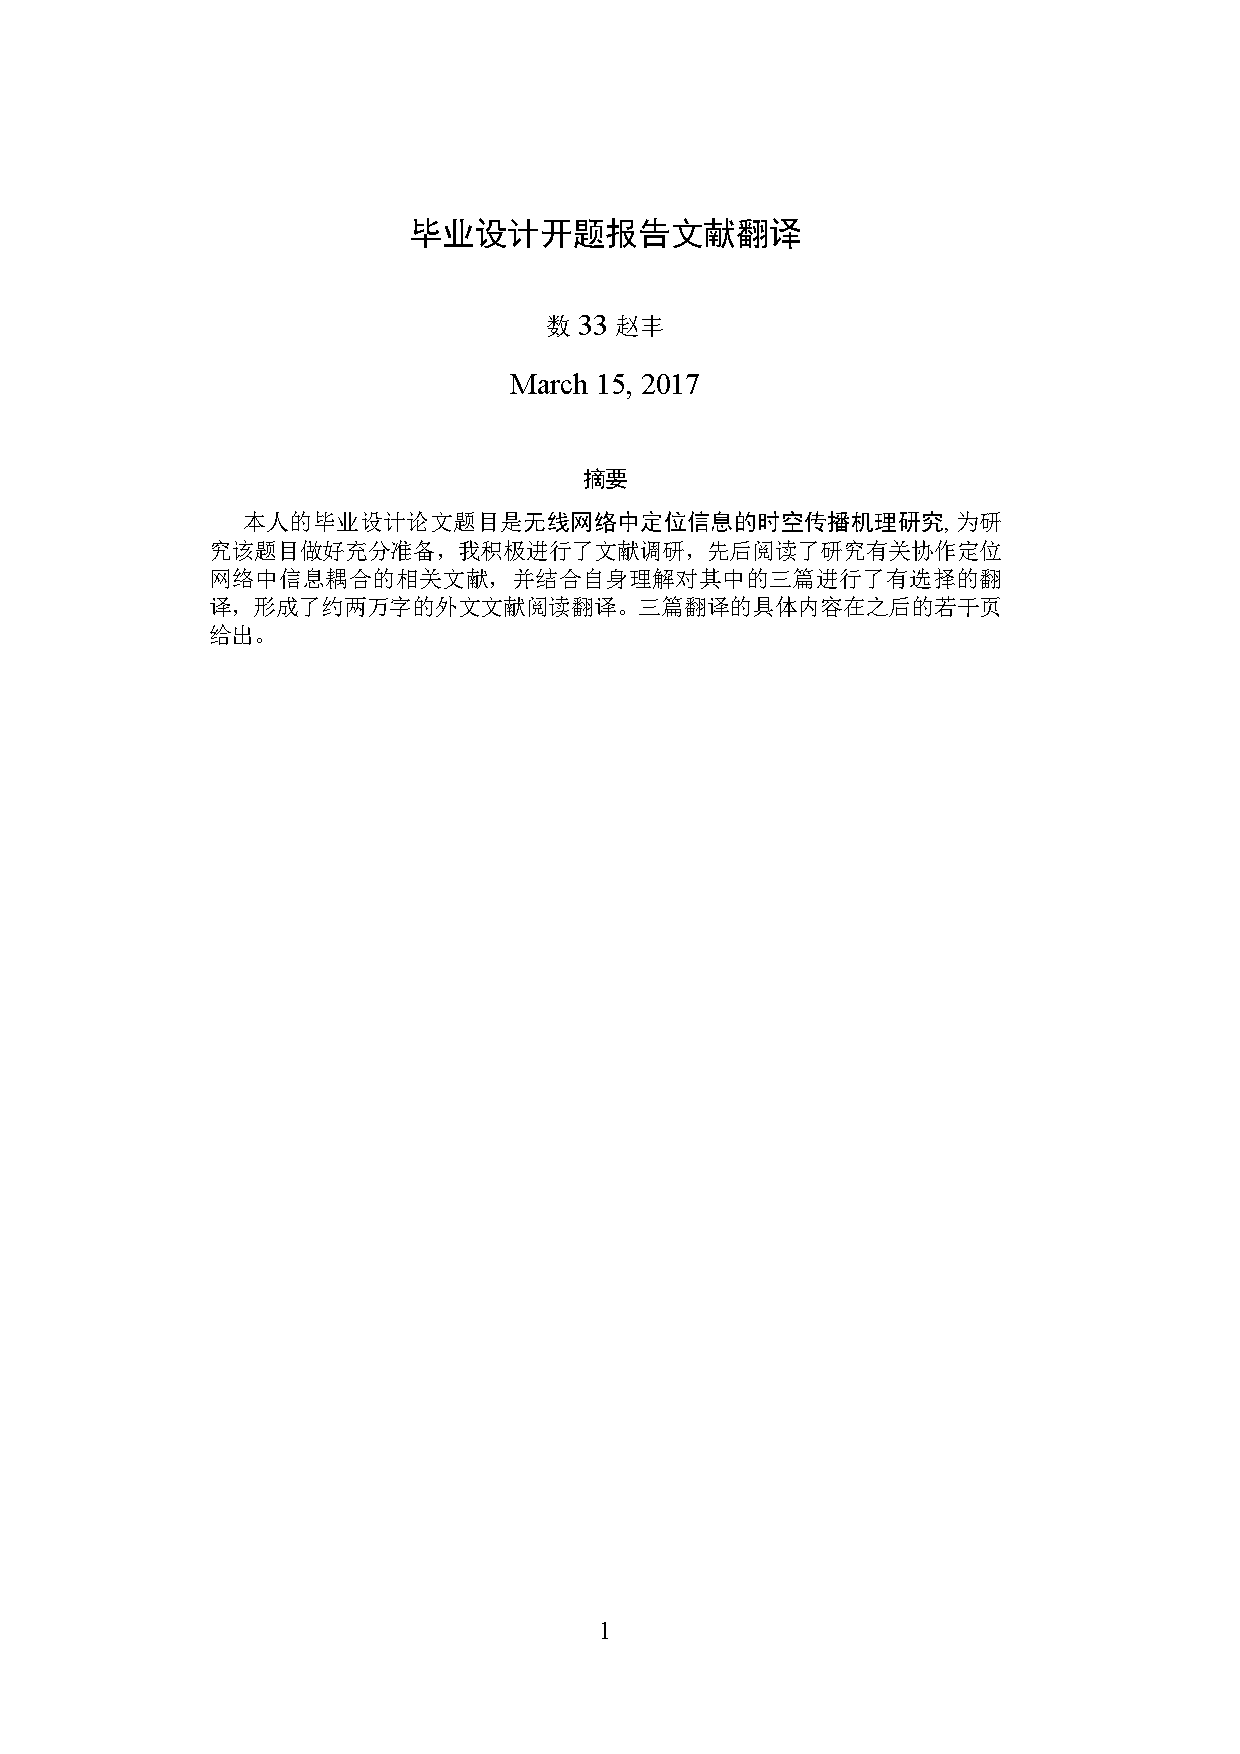
\includepdf[pages=-]{translation.pdf}
\chapter{公式的推导}
\section{建模过程的一些推导过程}
\subsection{定位问题中费舍尔信息矩阵一般结构推导}\label{A_F_1}
在非协作单节点定位中,测量量的联合概率分布由式(\ref{eq:single})给出,费舍尔信息矩阵是费舍尔信息量的自然推广,在满足一定正则性的条件下,费舍尔信息矩阵可以写成:
\begin{equation}
I(\bm{p})=-\mathbb{E}_{\bm{x}}(\bigtriangledown_{\bm{p}} \log f(\vec{x}|\bm{p}))^T(\bigtriangledown_{\bm{p}} \log f(\vec{x}|\bm{p}))
\end{equation}
其中f是随机向量$\vec{x}$的密度函数,利用上面的公式,首先对式(\ref{eq:single})取对数并求梯度得:
\begin{equation}
\bigtriangledown_{\bm{p}}\ln f=-\sum_{i=1}^{N_b}\frac{||\bm{p}_i^b-\bm{p}||-x_i}{\sigma_i^2}\frac{\bm{p}^b_i-\bm{p}}{||\bm{p}^b_i-\bm{p}||}
\end{equation}
注意到$\frac{||\bm{p}_i^b-\bm{p}||-x_i}{\sigma_i}\approx N(0,1)$,所以按照费舍尔信息矩阵的定义可得到式(\ref{eq:uu})的结果。
\section{研究成果的一些推导过程}
\subsection{两个未知节点协作最小误差界的一个充分条件}\label{B_F_0}
由式(\ref{eq:4_characteristic_polynomial}),SPEB为其所有根的倒数和,因此具有如下形式
\begin{equation}\label{eq:SPEB_GLOBAL}
\frac{\displaystyle\sum \frac{1}{\lambda_i}+\epsilon(\frac{\cos^2(\theta)}{\lambda_1}(\sum_{i \neq 1}\frac{1}{\lambda_i})+\frac{\sin^2(\theta)}{\lambda_2}(\displaystyle\sum_{i \neq 2}\frac{1}{\lambda_i})+\frac{\cos^2(\phi)}{\lambda_3}(\sum_{i \neq 3}\frac{1}{\lambda_i})+\frac{\sin^2(\phi)}{\lambda_4}(\sum_{i \neq 4}\frac{1}{\lambda_i}))}{\displaystyle 1+\epsilon(\frac{\cos^2(\theta)}{\lambda_1}+\frac{\sin^2(\theta)}{\lambda_2}+\frac{\cos^2(\phi)}{\lambda_3}+\frac{\sin^2(\phi)}{\lambda_4})}
\end{equation}
对固定的$\phi$,我们证明SPEB关于$\theta$是单调递减的。记$k=\frac{\cos^2 \theta}{a_1}+\frac{\sin^2 \theta}{a_2}$,$u=(\frac{1}{a_3}+\frac{1}{a_4}),v=(\frac{1}{a_1}+\frac{1}{a_2})$.~(\ref{eq:SPEB_GLOBAL})可以化为:
\begin{equation}
\text{SPEB}=u\frac{1+(\frac{1}{a_1}+\frac{1}{a_2})/u+\epsilon(\frac{1}{a_1a_2 u}+\frac{1}{a_3a_4 u}+k+(\frac{\cos^2\phi}{a_3}+\frac{\sin^2\phi}{a_4})\frac{v}{u})}{1+\epsilon(k+(\frac{\cos^2\phi}{a_3}+\frac{\sin^2\phi}{a_4}))}
\end{equation}
SPEB可以写成关于k的反比例函数$u\frac{A+k}{B+k}$的形式,其中
\[
A=(1+(\frac{1}{a_1}+\frac{1}{a_2})/u)/\epsilon+\frac{1}{a_1a_2 u}+\frac{1}{a_3a_4 u}+(\frac{\cos^2\phi}{a_3}+\frac{\sin^2\phi}{a_4})\frac{v}{u}
\]
\[
B=1/\epsilon+(\frac{\cos^2\phi}{a_3}+\frac{\sin^2\phi}{a_4})
\]
如果能证明$A \geq B$,那么该反比例函数关于k是单调递减的。
\[
A-B=(\frac{1}{a_1}+\frac{1}{a_2})/u\epsilon+\frac{1}{a_1a_2 u}+\frac{1}{a_3a_4 u}+(\frac{\cos^2\phi}{a_3}+\frac{\sin^2\phi}{a_4})(\frac{v}{u}-1)
\]
\[
\geq \frac{1}{a_3a_4 u}+(\frac{\cos^2\phi}{a_3}+\frac{\sin^2\phi}{a_4})(\frac{v}{u}-1)
\]
\[
=\frac{1}{u}((\frac{1}{a_1}+\frac{1}{a_2})(\frac{\cos^2\phi}{a_3}+\frac{\sin^2\phi}{a_4})-(\frac{\cos^2\phi}{a_3^2}+\frac{\sin^2\phi}{a_4^2}))
\]
由假设:$\frac{1}{a_1}+\frac{1}{a_2}\geq \max\{\frac{1}{a_4},\frac{1}{a_3}\}$
所以$A-B\geq 0$。
下面再证明k关于$\sin^2(\theta)$是单调递增的,那么由复合函数的单调性的性质,结论成立。
\[
k=\frac{1}{a_1}+\sin^2 \theta(\frac{1}{a_2}-\frac{1}{a_1})
\]
因为$a_1\geq a_2$所以在$\sin^2(\theta)\in[0,1]$的区间内结论成立。
同理可证明条件$\frac{1}{a_3}+\frac{1}{a_4}\geq \max\{\frac{1}{a_1},\frac{1}{a_2}\}$是保证固定$\theta$的情况下SPEB关于$\phi \in [0,\frac{\pi}{2}]$是单调递减的。
\subsection{单节点动态定位问题等效费舍尔信息矩阵推导}\label{B_F_1}
为简化符号,记$\bm{u}:=\bm{u}_{N_a-1}$,2阶单位阵记为$\bm{I}_2$,由等效费舍尔信息矩阵的定义,有
\begin{align}\notag\label{eq:initial_efim}
  U_{N_a}=&\lambda \bm{I}_2+\bm{u}\bm{u}^T-\bm{u}\bm{u}^T U_{N_a-1}^{-1}\bm{u}\bm{u}^T\\
  =&\lambda \bm{I}_2+(1-\bm{u}^T U_{N_a-1}^{-1}\bm{u})\bm{u}\bm{u}^T
\end{align}
因为$\bm{u}\bm{u}^T=U\begin{pmatrix}
                     1 & 0 \\
                     0 & 0
                   \end{pmatrix}U^{-1}$,其中$U$是由$\bm{u}$的方向角确定的二维旋转矩阵,所以
$U_{N_a}$相似于下面的矩阵
\[
U_{N_a}\sim \begin{pmatrix}
                           \lambda+1-\bm{u}^T U_{N_a-1}^{-1}\bm{u} & 0 \\
                           0 & \lambda
                         \end{pmatrix}
\]
                         
我们定义$T_i=\lambda+1-\bm{u}^T U_{N_a-i}^{-1}\bm{u}$并设$U_{N_a-1}=\bm{u}\bm{u}^T+J_2$
由式(\ref{eq:woodbury})可得
\begin{align}\notag
T_1=&\lambda+1-\bm{u}^T (\bm{u}\bm{u}^T+J_2)^{-1}\bm{u}\\
=&\lambda+(1+\bm{u}^T J_2^{-1}\bm{u})^{-1}
\end{align}
进一步设$v:=\bm{u}_{N_a-2}$,则$J_2=\lambda \bm{I}_2+(1-\bm{v}^T U_{N_a-2}^{-1}\bm{v})\bm{v}\bm{v}^T=V\begin{pmatrix}
                     \lambda+1-\bm{v}^T U_{N_a-2}^{-1}\bm{v} & 0 \\
                     0 & \lambda
                   \end{pmatrix}V^{-1}$
设$\bm{u}=(\cos\phi_1,\sin\phi_1)^T,\bm{v}=(\cos\phi_2,\sin\phi_2)^T$,则
\[
V^{-1}\bm{u}=\begin{pmatrix}
                     \cos\phi_2 & \sin\phi_2 \\
                     -\sin\phi_2 & \cos\phi_2
                   \end{pmatrix}\binom{\cos\phi_1}{\sin\phi_1}=\binom{\cos(\phi_1-\phi_2)}{\sin(\phi_1-\phi_2)}=:w
\]
所以
\begin{align*}
T_1=&\lambda+(1+\bm{w}^T \begin{pmatrix}
                     \lambda+1-\bm{v}^T U_{N_a-2}^{-1}\bm{v} & 0 \\
                     0 & \lambda
                   \end{pmatrix}^{-1}\bm{w})^{-1}\\
                   =&\frac{1}{1+\frac{\cos^2(\phi_1-\phi_2)}{T_2}+\frac{\sin^2(\phi_1-\phi_2)}{\lambda}}
\end{align*}
递推可得一般形式。
终止条件:
\begin{align*}
T_{N_a-1}&=\lambda+1-\bm{u}_1^T(\lambda\bm{I}+\bm{u}_1\bm{u}_1^T)^{-1}\bm{u}_1\\
&=\lambda+\frac{1}{\lambda+\frac{1}{\lambda}}
\end{align*}
\subsection{定理\ref{theorem:arbitrary_curve}的证明}\label{B_F_6}
式(\ref{eq:starting_or_ending})给出了式(\ref{eq:limiting_cf})右端是$\bm{p}(t)$为直线的情形。由于对于任意的平面曲线和角度序列$\{\theta_i\}$,$T_1(N_a)$是关于$N_a$的增函数且小于$\lambda+1$,因此式(\ref{eq:limiting_cf})左端的极限总是存在的。
考虑由$\bm{p}(t)$确定的角度序列$\{\theta_i\}$以如下的方式趋近于直线对应的直线序列:
\[
\{\theta_1,\theta_2,\theta_3,\dots\}\rightarrow\{0,\theta_2,\theta_3,\dots\}\rightarrow
\{0,0,\theta_3,\dots\}\rightarrow\dots
\]
记将前n个角度置零后由式(\ref{eq:recursive_efim})确定的连分式为$K_n$,我们首先给出:
\begin{equation}\label{eq:arbitrary_curve_1}
\lim_{n\to\infty}K_n=\frac{\lambda+\sqrt{4\lambda+\lambda^2}}{2}
\end{equation}
为证式(\ref{eq:arbitrary_curve_1}),记角度序列$\{0,0,\dots,\theta_{n+1},\dots,\}$去掉前r项后对应的连分式为$K^r_n$
\[
|K_n-M^*|=\frac{|\frac{1}{M^*}-\frac{1}{K^2_n}|}{(1+\frac{1}{M^*})(1+\frac{1}{K^2_n})}\leq |\frac{1}{M^*}-\frac{1}{K^2_n}|
\]
\[
|\frac{1}{M^*}-\frac{1}{K^2_n}|= \frac{|\frac{1}{M^*}-\frac{1}{K^3_n}|}{K^2_n(M^*+1)(1+\frac{1}{K^3_n})}=
 \frac{|\frac{1}{M^*}-\frac{1}{K^3_n}|}{(M^*+1)(\lambda+1+\frac{1}{K^3_n+1})}\leq \frac{|\frac{1}{M^*}-\frac{1}{K^3_n}|}{(\lambda+1)^2}
\]
当$r<n$ 时,
\[
|\frac{1}{M^*}-\frac{1}{K^r_n}|\leq \frac{|\frac{1}{M^*}-\frac{1}{K^{r+1}_n}|}{(\lambda+1)^2}
\]
因此:
\[
|K_n-M^*|\leq \frac{|\frac{1}{M^*}-\frac{1}{K^{n}_n}|}{(\lambda+1)^{2(n-2)}}
\]
故式(\ref{eq:arbitrary_curve_1})成立。
补充$K_0=\lim_{\Delta t\to 0}T_1(N_a)$这样式(\ref{eq:limiting_cf})即等价为
\begin{equation}\label{eq:equivalent_limiting_cf}
\sum_{i=1}^{\infty}(K_{i-1}-K_{i})=0
\end{equation}
先考虑$K_0-K_1$,二者的差别是$\theta_1$是否为0,
\[
K_0-K_1=\frac{1}{1+\frac{1}{K_1^1}}-\frac{1}{1+\frac{1}{K_1^1}+\sin^2\theta_1(\frac{1}{\lambda}-\frac{1}{K_1^1})}\leq
\sin^2\theta_1(\frac{1}{\lambda}-\frac{1}{K_1^1})
\]
类似式(\ref{eq:arbitrary_curve_1})的推导:
\[
K_r-K_{r+1}\leq \sin^2\theta_{r+1}(\frac{1}{\lambda}-\frac{1}{K_{r+1}^{r+1}})\frac{1}{(\lambda+1)^{2r}}
\]
由条件$\bm{p}'(t)$存在且连续可得切向量是连续变化的,由微分中值定理在闭区间内存在常数c使得角度变化量$\theta_i\leq c\Delta t$
由正弦函数的单调性推出:
\[
K_r-K_{r+1}\leq \sin^2 (c\Delta t) \frac{1}{\lambda}\frac{1}{(\lambda+1)^{2r}}
\]
因此
\begin{equation}\label{eq:quatratic_convergence}
0\leq \sum_{i=1}^{N_a}(K_{i-1}-K_{i})\leq \sin^2 (c\Delta t) \frac{1}{\lambda}\sum_{i=1}^{\infty}\frac{1}{(\lambda+1)^{2i}}
\end{equation}
无穷级数$\sum_{i=1}^{\infty}\frac{1}{(\lambda+1)^{2i}}$收敛,所以当$\Delta t\to 0$时$N_a\to \infty$,式(\ref{eq:equivalent_limiting_cf})成立。

\subsection{单节点动态定位问题等效费舍尔信息衰减上下界}\label{B_F_2}
为记号简便记$T'_1=T_1(N_a+1),T_1=T_1(N_a)$
%考虑在原有基础上增加一层节点,
%于是协作层数由原来的$N_a-1$变为$N_a$。等效费舍尔信息矩阵较大的特征值分别记为$T_1,T'_1$,
为便于比较,我们在$T_1$中引入虚拟节点将其层数也拓展为$N_a$,它只有锚点的定位信息,这样它们的区别是连分式的末端$T_{N_a}=\lambda$,$T'_{N_a}=\lambda+\frac{1}{1+1/\lambda}$
对$|T_1-T'_1|$从外向里通分得:
\[
|T_1-T'_1|=\frac{\cos^2\theta_1|\frac{1}{T_2}-\frac{1}{T'_2}|}{(1+\frac{\sin^2\theta_1}{\lambda}+\frac{\cos^2\theta_1}{T_2})
(1+\frac{\sin^2\theta_1}{\lambda}+\frac{\cos^2\theta_1}{T'_2})}\leq |\frac{1}{T_2}-\frac{1}{T'_2}|
\]
继续放缩$|\frac{1}{T_2}-\frac{1}{T'_2}|$有:
\[
|\frac{1}{T_2}-\frac{1}{T'_2}|= \frac{\cos^2\theta_2|\frac{1}{T_3}-\frac{1}{T'_3}|}{(1+\lambda(1+\frac{\sin^2\theta_2}{\lambda}+\frac{\cos^2\theta_2}{T_3}))
(1+\lambda(1+\frac{\sin^2\theta_2}{\lambda}+\frac{\cos^2\theta_2}{T'_3}))}\leq |\frac{1}{T_3}-\frac{1}{T'_3}|\frac{1}{(1+\lambda)^2}
\]
逐次递推得
\[
|T_1-T'_1|\leq \frac{1}{(1+\lambda)^{2(N_a-2)}} |\frac{1}{T_{N_a}}-\frac{1}{T'_{N_a}}|
\]
而:
\[
|\frac{1}{T_{N_a}}-\frac{1}{T'_{N_a}}|=\frac{1}{\lambda^2+2\lambda}
\]
另一方面,因为$T_2,T'_2\geq \lambda$
\[
|T_1-T'_1|\geq \frac{\cos^2\Delta\theta|\frac{1}{T_2}-\frac{1}{T'_2}|}{(1+1/\lambda)^2}
\]
\[
|\frac{1}{T_2}-\frac{1}{T'_2}|\geq \frac{\cos^2\Delta\theta|\frac{1}{T_3}-\frac{1}{T'_3}|}{(2+\lambda)^2}
\]
逐次递推得下界。
%\subsection{推论\ref{corollary:exponential_decreasing}的证明}\label{B_F_5}
%由定理\ref{theorem:exponential_decreasing}的结论:
%\[
%T_{N_a}=\sum_{k=1}^{N_a-1}\Delta_{+}T_k
%\]
%因此当$N_a\geq 2$时
%\[
%|T_{N_a}-T_{\infty}|=\sum_{k=N_a}^{\infty}\Delta_{+}T_k\leq %\frac{1}{\lambda^2+2\lambda}\sum_{k=N_a}^{\infty}\frac{1}{(\lambda+1)^{2(k-2)}}=\frac{1}{(\lambda^2+2\lambda)^2}\frac{1}{(\lambda+1)^{2(N_a-3)}}
%\]
%取$q=(\lambda+1)^2$,其余常数为C即可。
\subsection{单节点非均一测距误差等效费舍尔信息矩阵推导}\label{B_F_3}
类似式(\ref{eq:initial_efim})有:
\[
U_{N_a}=\bm{I}+(\lambda_1-\lambda_1^2 \bm{u}^T U_{N_a-1}^{-1}\bm{u})\bm{u}\bm{u}^T
\]
而
\[
T_1=1+\lambda_1-\lambda_1^2 \bm{u}^T U_{N_a-1}^{-1}\bm{u}=1+(\lambda_1^{-1}+\bm{u}^T\bm{J}_2^{-1}\bm{u})^{-1}
\]
对$J_2=\bm{I}_2+(\lambda_2-\lambda_2^2\bm{v}^T U_{N_a-2}^{-1}\bm{v})\bm{v}\bm{v}^T$提取关于$\bm{v}$的旋转矩阵即得到
式(\ref{eq:recursive_efim_second})。
另外从式(\ref{eq:recursive_efim_second})出发,设$\theta'_1\leq \theta_1$,作差:
\[
\text{denominator}~(T_1(\theta'_1)-T_1(\theta_1))=(\cos^2\theta'_1-\cos^2\theta_1)(1-\frac{1}{T_2})\geq 0
\]
即角度$\theta_1$越小$T_1$越大,同理$\theta_i$越小$T_i$越大,而由连分式的表达式可以看出$T_1$关于$T_2$递增,而连分式本身具有自相似性,
因此诸$\theta_i$减小可以增大信息量$T_1$。

\subsection{引理~\ref{lemma:hexagon}的推导}\label{B_F_4}
  设式(\ref{eq:equiv})左边为B,$A=\lambda+\frac{3}{2}$,那么由Woodbury矩阵求逆公式有
  \[
  (A+\frac{1}{\lambda+3/2-\frac{3/2}{\lambda+3/2}})^{-1}=A^{-1}-A^{-1}BA^{-1}
  \]
  整理得:
  \[
  B=A-\frac{A^2}{A+\frac{1}{\lambda+3/2-\frac{3/2}{\lambda+3/2}}}
  \]
  通分化简得证。
\section{本文中用到的关于连分式的结论}\label{C_F}
\begin{definition}
  有限序列$t_1,t_2,\dots,t_r$满足$t_j\geq 1$对于$j\geq2$可以递推地定义有限连分式
  \[[t_1,t_2,\dots,t_r]:=t_1+\frac{1} {[t_2,\dots,t_r]}\]
\end{definition}
\begin{theorem}\label{thm:basic}
  设$p_j=t_j p_{j-1}+p_{j-2},q_j=t_j q_{j-1}+q_{j-2}$,$M_j=\left(\begin{matrix}p_j&p_{j-1}\\q_j&q_{j-1}\end{matrix}\right)$
  $p_0,p_1,q_0,q_1$由$M_0=I_2$给出,且$T_j=\left(\begin{matrix}t_j&1\\1&0\end{matrix}\right)$则有下面三个恒等式:
  \begin{enumerate}
    \item $M_j=M_{j-1}T_j$
    \item $\binom{p_j}{q_j}=(\prod_{i=1}^r T_i )\binom{1}{0}$
    \item $[t_1,t_2,\dots,t_r]=\frac{p_r}{q_r}$
  \end{enumerate}
\end{theorem}
\begin{theorem}\label{theorem:quadratic_cyclic}
若$\lim_{r\to \infty}[t_1,t_2,\dots,t_r]$存在,该极限是形如$\frac{a+b\sqrt{m}}{c}$的二次根式当且仅当序列$t_i$从某项开始是周期的,即$\exists c,r,\,s.t.\, t_{i}=t_{i+r},\forall i\geq c$。
\end{theorem}
\begin{remark}
对于定理\ref{theorem:quadratic_cyclic},设$\left(\begin{matrix}a&b\\c&d\end{matrix}\right)=(\prod_{i=1}^{rc} T_{i+c})$,称$\left(\begin{matrix}a&b\\c&d\end{matrix}\right)$对应着分式线性变换K,如果$K(z)=\frac{az+b}{cz+d}$。
可以证明系数为实数的分式线性变换以函数复合作为群运算与行列式为1的2阶方阵以矩阵乘积作为群运算是同构的。
c之前的$t_i$对应着矩阵$T_i$的乘积矩阵看作分式线性变换F。可以进一步说明二次根式和T和F的有如下的关系:
\begin{enumerate}
  \item 首先求解$K$的不动点即解二次方程$x=\frac{ax+b}{cx+d}$得x
  \item $F(x)=\lim_{r\to \infty}[t_1,t_2,\dots,t_r]$,F(x)即为极限$\lim_{r\to \infty}[t_1,t_2,\dots,t_r]$
\end{enumerate}
一般二次方程有两个根,而有限连分式的极限值是唯一的,这时可根据极限值介于序列的前两个数之间剔除一个不合理的不动点。
\end{remark}

\end{appendix}


%% 本科生进行格式审查是需要下面这个表格,答辩可能不需要。选择性留下。
% 综合论文训练记录表
\includepdf[pages=-]{scan-record.pdf}
\end{document}
